
\documentclass[10pt]{article}

\usepackage[a4paper,margin=0.65in]{geometry}
\usepackage{amsmath,amssymb}
\usepackage{graphicx}
\usepackage{booktabs}
\usepackage{array}
\usepackage{float}
\usepackage{epstopdf}
\usepackage{adjustbox}
\usepackage{hyperref}
\usepackage{enumitem}
\usepackage{xcolor}
\usepackage{tikz}
\usetikzlibrary{positioning,arrows.meta,shapes.geometric,fit,calc}

\setlist{nosep,leftmargin=*}
\renewcommand{\arraystretch}{1.2}
\setlength{\parindent}{0pt}
\setlength{\parskip}{2pt}

\tikzset{
layer/.style={
draw,
rounded corners,
minimum width=1.7cm,
minimum height=0.65cm,
align=center,
fill=blue!10,
font=\scriptsize
},
smalllayer/.style={
draw,
rounded corners,
minimum width=1.35cm,
minimum height=0.58cm,
align=center,
fill=green!10,
font=\scriptsize
},
arrow/.style={
-{Latex[length=2mm]},
thin
}
}

\begin{document}

%%%%%%%%%%%%%%%%%%%%%%%%%%%%%%%%%%%%%%%%%%%%%%%%%%%%%%%%%%%%
% TITLE
%%%%%%%%%%%%%%%%%%%%%%%%%%%%%%%%%%%%%%%%%%%%%%%%%%%%%%%%%%%%

\begin{center}

{\large\textbf{Shiv Nadar University Chennai}}

\vspace{2mm}

{\normalsize\textbf{CS3807 -- Deep Learning Laboratory}}

\vspace{2mm}

{\large\textbf{Experiment 7}}

\vspace{1mm}

{\normalsize\textbf{End-to-End Study of Autoencoders, Convolutional}}

{\normalsize\textbf{Autoencoders, Denoising Autoencoders and Variational Autoencoders}}

\end{center}

\begin{flushleft}
\textbf{Name:} Johan Emmanuel S\\
\textbf{Registration Number:} 24011101043\\
\end{flushleft}

\vspace{3mm}

\begin{tabular}{|p{3.4cm}|p{9.0cm}|p{1.4cm}|}
\hline
Degree \& Branch &
B.Tech Artificial Intelligence \& Data Science &
Semester V\\
\hline
Subject Code \& Name &
CS3807 -- Deep Learning Laboratory &
AY: 2026--27\\
\hline
\end{tabular}

%%%%%%%%%%%%%%%%%%%%%%%%%%%%%%%%%%%%%%%%%%%%%%%%%%%%%%%%%%%%
\section*{1. Objective}

The objective of this experiment is to develop an end-to-end understanding of
autoencoders and their variants for image representation, reconstruction,
denoising and generative modeling.

The experiment begins with a fully connected autoencoder, progresses to a
Convolutional Autoencoder (CAE), introduces image corruption for denoising,
and finally develops a Variational Autoencoder (VAE). Students will visualize
the learned latent representation, compare reconstruction quality using
quantitative and qualitative measures, and explore the generative capability
of the VAE.

The same image dataset and a controlled experimental protocol should be used
throughout the experiment wherever possible.

%%%%%%%%%%%%%%%%%%%%%%%%%%%%%%%%%%%%%%%%%%%%%%%%%%%%%%%%%%%%
\section*{2. Learning Outcomes}

After completing this experiment, students will be able to:

\begin{itemize}
\item explain the encoder--latent--decoder structure of an autoencoder;
\item prepare image data for reconstruction-based learning;
\item implement a fully connected autoencoder;
\item implement a Convolutional Autoencoder for image reconstruction;
\item introduce controlled noise and build a denoising autoencoder;
\item evaluate reconstruction using MSE, MAE and SSIM;
\item visualize and interpret latent representations;
\item explain the probabilistic latent representation of a VAE;
\item implement the reparameterization trick;
\item calculate and interpret reconstruction and KL-divergence losses;
\item generate new images by sampling from a learned latent space; and
\item compare deterministic and variational latent representations.
\end{itemize}

%%%%%%%%%%%%%%%%%%%%%%%%%%%%%%%%%%%%%%%%%%%%%%%%%%%%%%%%%%%%
\section*{3. Dataset and Experimental Setup}

\textbf{Dataset: MNIST Handwritten Digit Dataset}

MNIST contains grayscale images of handwritten digits from 0 to 9. Each image
has spatial dimensions

\[
28\times28\times1.
\]

The dataset is particularly suitable for this experiment because the images
are small, the classes have visually meaningful structure, and the same image
format can be directly supplied to fully connected, convolutional and
variational autoencoders.

The dataset can be loaded directly using Keras/TensorFlow:

\url{https://www.tensorflow.org/api_docs/python/tf/keras/datasets/mnist}

\textbf{Recommended laboratory subset:}

Use 10,000 training images and 2,000 test images for the main laboratory
execution. The full MNIST dataset may be used if computational resources
permit.

The labels are not required as reconstruction targets. The original image is
the target:

\[
\boxed{x\rightarrow \text{Encoder}\rightarrow z
\rightarrow\text{Decoder}\rightarrow\hat{x}}
\]

where $x$ is the input image and $\hat{x}$ is its reconstruction.

%%%%%%%%%%%%%%%%%%%%%%%%%%%%%%%%%%%%%%%%%%%%%%%%%%%%%%%%%%%%
\section*{4. Expected Input and Output}

\subsection*{Expected Input}

Each input image has shape

\[
28\times28\times1.
\]

For a batch of 32 images:

\[
X\in\mathbb{R}^{32\times28\times28\times1}.
\]

Pixel values should be converted from

\[
[0,255]\rightarrow[0,1].
\]

For a fully connected autoencoder, the image may be flattened:

\[
28\times28=784.
\]

Therefore,

\[
x\in\mathbb{R}^{784}.
\]

For a convolutional autoencoder, retain the spatial structure:

\[
x\in\mathbb{R}^{28\times28\times1}.
\]

\subsection*{Expected Output}

The primary output is a reconstructed image:

\[
\hat{x}\in\mathbb{R}^{28\times28\times1}.
\]

Students must display:

\begin{verbatim}
Original image
Reconstructed image
Reconstruction error
\end{verbatim}

For the denoising model, display:

\begin{verbatim}
Original clean image
Noisy image
Denoised reconstruction
\end{verbatim}

For the VAE, display newly generated samples obtained by sampling from the
latent distribution.

%%%%%%%%%%%%%%%%%%%%%%%%%%%%%%%%%%%%%%%%%%%%%%%%%%%%%%%%%%%%
\section*{5. Overall Experimental Pipeline}

The complete experiment follows:

\begin{center}
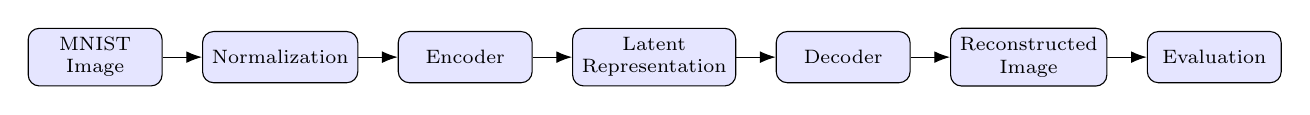
\begin{tikzpicture}[node distance=5mm]
\node[layer](a){MNIST\\Image};
\node[layer,right=of a](b){Normalization};
\node[layer,right=of b](c){Encoder};
\node[layer,right=of c](d){Latent\\Representation};
\node[layer,right=of d](e){Decoder};
\node[layer,right=of e](f){Reconstructed\\Image};
\node[layer,right=of f](g){Evaluation};

\foreach \x/\y in {a/b,b/c,c/d,d/e,e/f,f/g}
\draw[arrow](\x)--(\y);
\end{tikzpicture}
\end{center}

The experiment consists of four related studies:

\begin{enumerate}
\item Fully Connected Autoencoder
\item Convolutional Autoencoder
\item Denoising Convolutional Autoencoder
\item Variational Autoencoder
\end{enumerate}

%%%%%%%%%%%%%%%%%%%%%%%%%%%%%%%%%%%%%%%%%%%%%%%%%%%%%%%%%%%%
\section*{6. Exploring Autoencoders}

An autoencoder learns to reproduce its input at the output.

The encoder maps the input to a lower-dimensional representation:

\[
z=f_{\theta}(x),
\]

and the decoder reconstructs the input:

\[
\hat{x}=g_{\phi}(z).
\]

The training objective is to minimize reconstruction error:

\[
\mathcal{L}_{rec}
=
\frac{1}{N}\sum_{i=1}^{N}
\|x_i-\hat{x}_i\|^2.
\]

\begin{center}
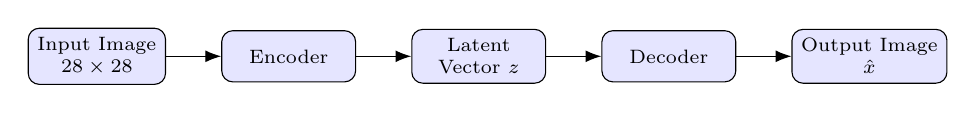
\begin{tikzpicture}[node distance=7mm]
\node[layer](a){Input Image\\$28\times28$};
\node[layer,right=of a](b){Encoder};
\node[layer,right=of b](c){Latent\\Vector $z$};
\node[layer,right=of c](d){Decoder};
\node[layer,right=of d](e){Output Image\\$\hat{x}$};

\foreach \x/\y in {a/b,b/c,c/d,d/e}
\draw[arrow](\x)--(\y);
\end{tikzpicture}
\end{center}

The latent vector is a compressed representation of the input.

%%%%%%%%%%%%%%%%%%%%%%%%%%%%%%%%%%%%%%%%%%%%%%%%%%%%%%%%%%%%
\section*{7. Fully Connected Autoencoder}

Flatten each image from

\[
28\times28=784
\]

to a vector of length 784.

Use the following architecture:

\begin{center}
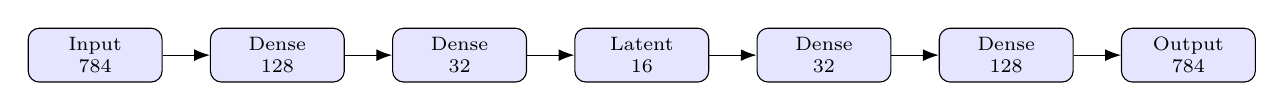
\begin{tikzpicture}[node distance=6mm]
\node[layer](a){Input\\784};
\node[layer,right=of a](b){Dense\\128};
\node[layer,right=of b](c){Dense\\32};
\node[layer,right=of c](d){Latent\\16};
\node[layer,right=of d](e){Dense\\32};
\node[layer,right=of e](f){Dense\\128};
\node[layer,right=of f](g){Output\\784};

\foreach \x/\y in {a/b,b/c,c/d,d/e,e/f,f/g}
\draw[arrow](\x)--(\y);
\end{tikzpicture}
\end{center}

Use ReLU activation in hidden layers and sigmoid activation in the output
layer.

\textbf{Suggested configuration:}

\begin{center}
\begin{tabular}{|l|l|}
\hline
Parameter & Value\\
\hline
Latent dimension & 16\\
Optimizer & Adam\\
Learning rate & $10^{-3}$\\
Batch size & 128\\
Epochs & 20\\
Loss & Binary Cross-Entropy\\
\hline
\end{tabular}
\end{center}

%%%%%%%%%%%%%%%%%%%%%%%%%%%%%%%%%%%%%%%%%%%%%%%%%%%%%%%%%%%%
\section*{8. Required Analysis of the Basic Autoencoder}

\textbf{Plot 1: Original versus Reconstructed Images}

\begin{figure}[H]
\centering
\includegraphics[width=0.95\linewidth]{original_vs_reconstructed.eps}
\caption{Plot 1: Original (top) versus fully connected AE reconstruction (bottom) for 10 test images.}
\end{figure}

\textbf{Inference:} The overall digit shape is preserved for all ten images, with simple digits (1, 0, 7) reconstructed almost sharply. Fine strokes and closed loops are blurred for complex digits (4, 9, 5), and the sample at position 8 (a hooked 9) is the worst, since a 16-dimensional dense bottleneck keeps only coarse structure.

\textbf{Plot 2: Training and Validation Reconstruction Loss}

\begin{itemize}
\item X-axis: Epoch
\item Y-axis: Reconstruction loss
\item Curves: Training loss and validation loss
\end{itemize}

\begin{figure}[H]
\centering
\includegraphics[width=0.6\linewidth]{reconstruction_loss_curve.eps}
\caption{Plot 2: Training and validation reconstruction loss (BCE) of the fully connected AE over 20 epochs.}
\end{figure}

\textbf{Inference:} Training loss falls from 0.344 to 0.120 and validation loss from 0.242 to 0.124, so the model converges smoothly. The two curves stay very close (final gap $\approx$0.004), so there is no overfitting; both are still decreasing slowly, suggesting more epochs could help slightly.

%%%%%%%%%%%%%%%%%%%%%%%%%%%%%%%%%%%%%%%%%%%%%%%%%%%%%%%%%%%%
\section*{9. Reconstruction Metrics}

Students must calculate the following metrics on the test set.

\subsection*{Mean Squared Error}

\[
MSE=
\frac{1}{N}
\sum_{i=1}^{N}
(x_i-\hat{x}_i)^2.
\]

\subsection*{Mean Absolute Error}

\[
MAE=
\frac{1}{N}
\sum_{i=1}^{N}
|x_i-\hat{x}_i|.
\]

\subsection*{Structural Similarity}

Calculate SSIM between the original and reconstructed images.

The implementation may use:

\url{https://scikit-image.org/docs/stable/api/skimage.metrics.html}

Report:

\begin{center}
\begin{tabular}{|l|c|}
\hline
Metric & Value\\
\hline
Test MSE & 0.020998\\
Test MAE & 0.055382\\
Mean SSIM & 0.751880\\
\hline
\end{tabular}
\end{center}

%%%%%%%%%%%%%%%%%%%%%%%%%%%%%%%%%%%%%%%%%%%%%%%%%%%%%%%%%%%%
\section*{10. Convolutional Autoencoder}

A Convolutional Autoencoder preserves spatial structure and uses convolutional
operations in the encoder and upsampling/transposed convolution operations
in the decoder.

The conceptual architecture is:

\begin{center}
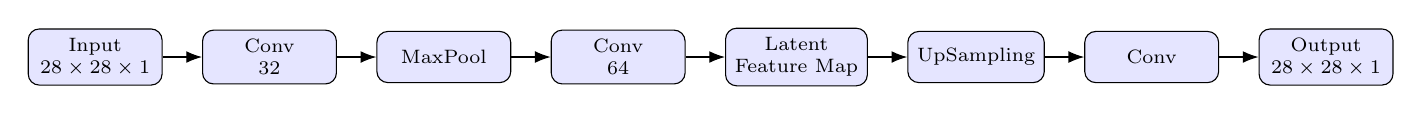
\begin{tikzpicture}[node distance=5mm]
\node[layer](a){Input\\$28\times28\times1$};
\node[layer,right=of a](b){Conv\\32};
\node[layer,right=of b](c){MaxPool};
\node[layer,right=of c](d){Conv\\64};
\node[layer,right=of d](e){Latent\\Feature Map};
\node[layer,right=of e](f){UpSampling};
\node[layer,right=of f](g){Conv};
\node[layer,right=of g](h){Output\\$28\times28\times1$};

\foreach \x/\y in {a/b,b/c,c/d,d/e,e/f,f/g,g/h}
\draw[arrow](\x)--(\y);
\end{tikzpicture}
\end{center}

A possible implementation is:

\begin{verbatim}
Input(28,28,1)
Conv2D(32, 3, activation='relu', padding='same')
MaxPooling2D(2, padding='same')
Conv2D(64, 3, activation='relu', padding='same')
MaxPooling2D(2, padding='same')
Conv2D(64, 3, activation='relu', padding='same')
UpSampling2D(2)
Conv2D(32, 3, activation='relu', padding='same')
UpSampling2D(2)
Conv2D(1, 3, activation='sigmoid', padding='same')
\end{verbatim}

The exact implementation may use Conv2DTranspose instead of UpSampling2D.

%%%%%%%%%%%%%%%%%%%%%%%%%%%%%%%%%%%%%%%%%%%%%%%%%%%%%%%%%%%%
\section*{11. Comparing Fully Connected and Convolutional Autoencoders}

Train both models using the same training and test images.

\begin{center}
\begin{tabular}{|l|c|c|c|c|}
\hline
Model & MSE & MAE & SSIM & Parameters\\
\hline
Fully Connected AE & 0.020998 & 0.055382 & 0.751880 & 211,040\\
Convolutional AE & 0.002506 & 0.014868 & 0.974898 & 74,497\\
\hline
\end{tabular}
\end{center}

\textbf{Plot 3: Reconstruction Comparison}

\begin{figure}[H]
\centering
\includegraphics[width=0.95\linewidth]{reconstruction_comparison.eps}
\caption{Plot 3: Original (top), FC-AE (middle) and CAE (bottom) reconstructions of 10 test images.}
\end{figure}

\textbf{Inference:} The CAE reconstructions are almost indistinguishable from the originals, whereas the FC-AE outputs are blurry and distort difficult digits. Convolution shares local filters and keeps the 7$\times$7$\times$64 spatial feature map, so edges and strokes are preserved; the CAE reduces MSE about 8$\times$ (0.0210 $\to$ 0.0025) and raises SSIM from 0.75 to 0.97 with 65\% fewer parameters.

%%%%%%%%%%%%%%%%%%%%%%%%%%%%%%%%%%%%%%%%%%%%%%%%%%%%%%%%%%%%
\section*{12. Denoising Autoencoder}

A denoising autoencoder receives a corrupted image but is trained to
reconstruct the original clean image.

The training mapping is:

\[
\boxed{\tilde{x}\rightarrow\text{Encoder}\rightarrow z
\rightarrow\text{Decoder}\rightarrow\hat{x}}
\]

where $\tilde{x}$ is a noisy version of the clean image $x$.

\begin{center}
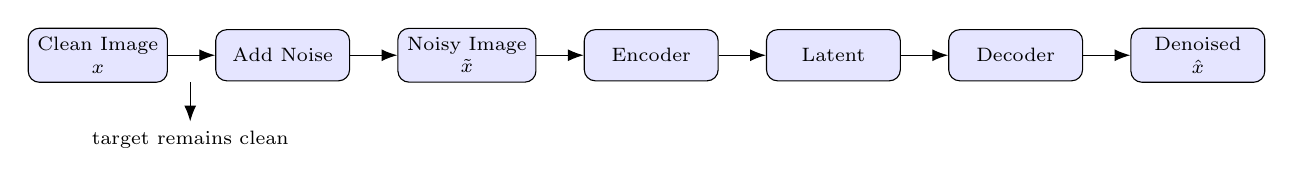
\begin{tikzpicture}[node distance=6mm]
\node[layer](a){Clean Image\\$x$};
\node[layer,right=of a](b){Add Noise};
\node[layer,right=of b](c){Noisy Image\\$\tilde{x}$};
\node[layer,right=of c](d){Encoder};
\node[layer,right=of d](e){Latent};
\node[layer,right=of e](f){Decoder};
\node[layer,right=of f](g){Denoised\\$\hat{x}$};

\foreach \x/\y in {a/b,b/c,c/d,d/e,e/f,f/g}
\draw[arrow](\x)--(\y);

\draw[arrow]($(a.south)!0.5!(b.south)$) -- ++(0,-5mm)
node[below,font=\scriptsize]{target remains clean};
\end{tikzpicture}
\end{center}

%%%%%%%%%%%%%%%%%%%%%%%%%%%%%%%%%%%%%%%%%%%%%%%%%%%%%%%%%%%%
\section*{13. Adding Image Noise}

Use at least two corruption types.

\subsection*{Gaussian Noise}

\[
\tilde{x}=x+n,
\qquad
n\sim\mathcal{N}(0,\sigma^2).
\]

Suggested standard deviations:

\[
\sigma\in\{0.1,0.2,0.3\}.
\]

Clip the resulting image to the range $[0,1]$.

\subsection*{Salt-and-Pepper Noise}

Randomly replace a small proportion of pixels with values close to 0 or 1.

Suggested corruption levels:

\[
p\in\{0.05,0.10,0.20\}.
\]

%%%%%%%%%%%%%%%%%%%%%%%%%%%%%%%%%%%%%%%%%%%%%%%%%%%%%%%%%%%%
\section*{14. Required Denoising Plots}

\textbf{Plot 4: Clean vs. Noisy vs. Denoised}

\begin{figure}[H]
\centering
\includegraphics[width=0.95\linewidth]{clean_vs_noisy_vs_denoised.eps}
\caption{Plot 4: Clean (top), Gaussian-noisy with $\sigma=0.2$ (middle) and denoised by the CDAE (bottom).}
\end{figure}

\textbf{Inference:} The noisy images show a grainy background and broken strokes, while the denoised outputs have a clean black background and continuous strokes. The CDAE recovers the full digit structure for all ten samples, with only slight thinning or smoothing of stroke edges.

\textbf{Plot 5: Noise Level vs. Reconstruction Quality}

For each noise level, calculate:

\[
MSE,\quad MAE,\quad SSIM.
\]

Report:

\begin{center}
\begin{tabular}{|c|c|c|c|}
\hline
Noise Level & MSE & MAE & SSIM\\
\hline
0.1 & 0.003813 & 0.018184 & 0.958773\\
0.2 & 0.004775 & 0.021443 & 0.944068\\
0.3 & 0.007161 & 0.029384 & 0.868043\\
\hline
\end{tabular}
\end{center}

{\footnotesize Note: each noise level uses a fresh random noise draw on the test set with the CDAE trained at $\sigma=0.2$, so the $\sigma=0.2$ row differs slightly from the Denoising CAE row in Section 21 (a different draw).}

\begin{figure}[H]
\centering
\includegraphics[width=0.6\linewidth]{noise_level_vs_reconstruction_quality.eps}
\caption{Plot 5: Noise level ($\sigma$) versus MSE, MAE (left axis) and SSIM (right axis) for the CDAE trained at $\sigma=0.2$.}
\end{figure}

\textbf{Inference:} MSE and MAE rise and SSIM falls as $\sigma$ increases, with a sharper degradation at $\sigma=0.3$ (SSIM 0.87), since heavier corruption destroys more pixel information and exceeds the noise level seen in training. Even so, SSIM stays above 0.86 at every level, so the major digit structure is still recovered.

%%%%%%%%%%%%%%%%%%%%%%%%%%%%%%%%%%%%%%%%%%%%%%%%%%%%%%%%%%%%
\section*{15. Variational Autoencoder}

A conventional autoencoder maps an input to a deterministic latent vector:

\[
z=f(x).
\]

A VAE instead learns a probability distribution:

\[
q_{\phi}(z|x)
=
\mathcal{N}
\left(
\mu(x),
\operatorname{diag}(\sigma^2(x))
\right).
\]

The encoder produces:

\[
\mu,\qquad \log\sigma^2.
\]

A latent vector is sampled using the reparameterization trick:

\[
z=\mu+\sigma\odot\epsilon,
\qquad
\epsilon\sim\mathcal{N}(0,I).
\]

\begin{center}
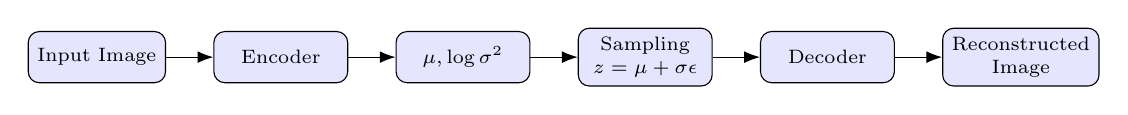
\begin{tikzpicture}[node distance=6mm]
\node[layer](a){Input Image};
\node[layer,right=of a](b){Encoder};
\node[layer,right=of b](c){$\mu,\log\sigma^2$};
\node[layer,right=of c](d){Sampling\\$z=\mu+\sigma\epsilon$};
\node[layer,right=of d](e){Decoder};
\node[layer,right=of e](f){Reconstructed\\Image};

\foreach \x/\y in {a/b,b/c,c/d,d/e,e/f}
\draw[arrow](\x)--(\y);
\end{tikzpicture}
\end{center}

%%%%%%%%%%%%%%%%%%%%%%%%%%%%%%%%%%%%%%%%%%%%%%%%%%%%%%%%%%%%
\section*{16. VAE Loss Function}

The VAE objective consists of two components.

\subsection*{Reconstruction Loss}

\[
\mathcal{L}_{rec}
=
-\mathbb{E}_{q_{\phi}(z|x)}
[\log p_{\theta}(x|z)].
\]

For normalized MNIST images, binary cross-entropy can be used.

\subsection*{KL Divergence}

\[
D_{KL}
\left(
q_{\phi}(z|x)\parallel p(z)
\right)
=
-\frac{1}{2}
\sum_j
\left(
1+\log\sigma_j^2-\mu_j^2-\sigma_j^2
\right).
\]

The total loss is

\[
\boxed{
\mathcal{L}_{VAE}
=
\mathcal{L}_{rec}
+
\mathcal{L}_{KL}
}
\]

where the prior is usually

\[
p(z)=\mathcal{N}(0,I).
\]

%%%%%%%%%%%%%%%%%%%%%%%%%%%%%%%%%%%%%%%%%%%%%%%%%%%%%%%%%%%%
\section*{17. VAE Implementation}

Use a small latent space so that it can be visualized.

Suggested latent dimension:

\[
z\in\mathbb{R}^{2}.
\]

The encoder should produce:

\[
\mu\in\mathbb{R}^{2},
\qquad
\log\sigma^2\in\mathbb{R}^{2}.
\]

The decoder maps

\[
z\rightarrow28\times28\times1.
\]

A compact architecture is:

\begin{center}
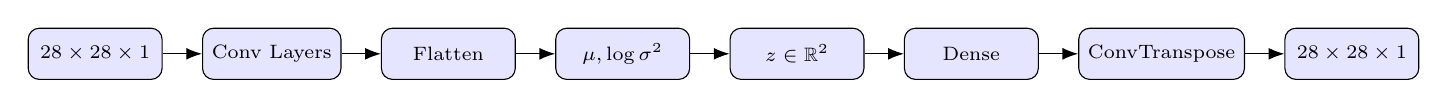
\begin{tikzpicture}[node distance=5mm]
\node[layer](a){$28\times28\times1$};
\node[layer,right=of a](b){Conv Layers};
\node[layer,right=of b](c){Flatten};
\node[layer,right=of c](d){$\mu,\log\sigma^2$};
\node[layer,right=of d](e){$z\in\mathbb{R}^2$};
\node[layer,right=of e](f){Dense};
\node[layer,right=of f](g){ConvTranspose};
\node[layer,right=of g](h){$28\times28\times1$};

\foreach \x/\y in {a/b,b/c,c/d,d/e,e/f,f/g,g/h}
\draw[arrow](\x)--(\y);
\end{tikzpicture}
\end{center}

%%%%%%%%%%%%%%%%%%%%%%%%%%%%%%%%%%%%%%%%%%%%%%%%%%%%%%%%%%%%
\section*{18. Exploring the VAE Latent Space}

Since the latent dimension is two, students can visualize the encoded test
images in a two-dimensional plane.

\textbf{Plot 6: VAE Latent Space}

\begin{itemize}
\item X-axis: $z_1$
\item Y-axis: $z_2$
\item Color/marker category: digit label
\end{itemize}

The labels are used only for visualization; they are not supplied to the VAE
during training.

\begin{figure}[H]
\centering
\includegraphics[width=0.7\linewidth]{vae_latent_space.eps}
\caption{Plot 6: 2-D VAE latent space ($\mu$ of 2000 test images) coloured by digit label.}
\end{figure}

\textbf{Inference:} Digits 1 (far left), 0 (lower right) and 7 (top) form well-separated clusters, and 6 occupies its own lower-central region. Digits 2, 3, 5 and 8 overlap heavily near the origin, and 4 and 9 overlap each other, because they are visually similar and only two dimensions are available. The latent cloud is centred near the origin with unit-scale spread, consistent with the $\mathcal{N}(0,I)$ prior.

%%%%%%%%%%%%%%%%%%%%%%%%%%%%%%%%%%%%%%%%%%%%%%%%%%%%%%%%%%%%
\section*{19. Generating New Images with the VAE}

Sample points from

\[
z\sim\mathcal{N}(0,I).
\]

Pass the sampled latent vectors through the decoder.

\textbf{Plot 7: Randomly Generated Images}

\begin{figure}[H]
\centering
\includegraphics[width=0.6\linewidth]{vae_generated_images.eps}
\caption{Plot 7: 25 images generated by decoding $z\sim\mathcal{N}(0,I)$.}
\end{figure}

\textbf{Inference:} Most samples are recognisable digits (0, 1, 7, 8, 9) with visible variation in slant, thickness and style. Some samples (e.g., blobs in rows 2 and 5) are ambiguous, and all are blurry, since the 2-D latent space is tiny and regions between clusters decode to blended shapes.

%%%%%%%%%%%%%%%%%%%%%%%%%%%%%%%%%%%%%%%%%%%%%%%%%%%%%%%%%%%%
\section*{20. Latent Space Interpolation}

Select two latent vectors:

\[
z_A,\qquad z_B.
\]

Construct

\[
z(\alpha)=(1-\alpha)z_A+\alpha z_B,
\qquad
\alpha\in[0,1].
\]

Use values such as:

\[
\alpha=
0,\;0.1,\;0.2,\ldots,1.
\]

Decode every interpolated vector.

\textbf{Plot 8: Latent Space Interpolation}

\begin{figure}[H]
\centering
\includegraphics[width=0.95\linewidth]{latent_space_interpolation.eps}
\caption{Plot 8: Decoded images along $z(\alpha)$ from a digit 0 ($\alpha=0$) to a digit 1 ($\alpha=1$).}
\end{figure}

\textbf{Inference:} The image changes gradually and continuously: the 0 loop narrows for $\alpha\le0.3$, passes through an ambiguous blob near $\alpha\approx0.4$--$0.5$, and becomes a clean slanted 1 from $\alpha\ge0.6$. The absence of abrupt jumps shows the VAE latent space is smooth and continuous, which is the result of the KL regularisation.

%%%%%%%%%%%%%%%%%%%%%%%%%%%%%%%%%%%%%%%%%%%%%%%%%%%%%%%%%%%%
\section*{21. Reconstruction Comparison Across Models}

Comparison the three reconstruction-based models:

\begin{center}
\begin{tabular}{|l|c|c|c|c|}
\hline
Model & MSE & MAE & SSIM & Parameters\\
\hline
Fully Connected AE & 0.020998 & 0.055382 & 0.751880 & 211,040\\
Convolutional AE & 0.002506 & 0.014868 & 0.974898 & 74,497\\
Denoising CAE & 0.004799 & 0.021508 & 0.943831 & 74,497\\
\hline
\end{tabular}
\end{center}

{\footnotesize The VAE reconstruction and KL losses are summed over pixels and latent dimensions, per image (nats), so they are not comparable with the per-pixel BCE of the other models.}

\begin{center}
\begin{tabular}{|l|c|}
\hline
VAE Metric & Value\\
\hline
Reconstruction Loss & 150.019608\\
KL Loss & 5.562951\\
Total Loss & 155.582535\\
Test MSE & 0.043855\\
Test MAE & 0.102490\\
Mean SSIM & 0.485874\\
\hline
\end{tabular}
\end{center}

\begin{figure}[H]
\centering
\includegraphics[width=0.6\linewidth]{vae_reconstruction_loss_curve.eps}
\caption{Plot: VAE training and validation reconstruction loss (summed BCE per image) over 20 epochs.}
\end{figure}

\textbf{Inference:} Training reconstruction loss drops from 293.7 to 149.3 and validation loss from 205.3 to 150.0, and the curves nearly coincide after about epoch 10. The VAE converges without overfitting; the total loss is dominated by reconstruction (KL $\approx$5.6).

%%%%%%%%%%%%%%%%%%%%%%%%%%%%%%%%%%%%%%%%%%%%%%%%%%%%%%%%%%%%
\section*{22. Reconstruction Error Distribution}

Calculate the per-image reconstruction error:

\[
e_i=
\frac{1}{D}
\sum_{j=1}^{D}
(x_{ij}-\hat{x}_{ij})^2.
\]

\textbf{Plot 9: Distribution of Reconstruction Errors}

\begin{figure}[H]
\centering
\includegraphics[width=0.6\linewidth]{reconstruction_error_distribution.eps}
\caption{Plot 9: Histogram of per-image reconstruction MSE of the VAE on the 2000 test images.}
\end{figure}

\textbf{Inference:} Most errors lie between 0.03 and 0.06 (mean 0.0439, median 0.0444), with a small low-error mode near 0.01 (simple digits such as 1) and a right tail up to about 0.12. The spread is moderate, and the high-error tail holds complex, thick or unusual digits that a 2-D latent space cannot encode.

%%%%%%%%%%%%%%%%%%%%%%%%%%%%%%%%%%%%%%%%%%%%%%%%%%%%%%%%%%%%
\section*{23. Required High-Error Image Analysis}

\begin{figure}[H]
\centering
\includegraphics[width=0.6\linewidth]{top5_high_error_samples.eps}
\caption{The five test images having the largest reconstruction errors.}
\end{figure}

\textbf{Test-set indices and per-image MSE:} 1352 (0.1210), 1847 (0.1153), 998 (0.1153), 864 (0.1116), 810 (0.1084).

\textbf{Inference:} These are unusual handwriting styles: a looped, thick 2, a 5 with a large closed bottom loop, two heavily filled 8s, and a crossed 7. The 2-D VAE bottleneck decodes them into blurry average shapes (often a 3/8-like blob), since such styles are rare in training and their many filled pixels give large squared errors.

%%%%%%%%%%%%%%%%%%%%%%%%%%%%%%%%%%%%%%%%%%%%%%%%%%%%%%%%%%%%
\section*{24. Consolidated Results}

\begin{center}
\begin{tabular}{|l|c|c|c|c|c|}
\hline
Model & MSE & MAE & SSIM & Parameters & Time\\
\hline
FC Autoencoder & 0.020998 & 0.055382 & 0.751880 & 211,040 & 0.2192 s\\
Conv. Autoencoder & 0.002506 & 0.014868 & 0.974898 & 74,497 & 0.2186 s\\
Denoising CAE & 0.004799 & 0.021508 & 0.943831 & 74,497 & 0.2205 s\\
VAE & 0.043855 & 0.102490 & 0.485874 & 284,933 & 0.4418 s\\
\hline
\end{tabular}
\end{center}

\textbf{Inference:} The CAE is the best reconstruction model (lowest MSE, highest SSIM) with the fewest parameters, and the Denoising CAE is close behind despite receiving noisy inputs. The VAE has the weakest pixel-level scores because its 2-D stochastic bottleneck and KL regularisation trade fidelity for a smooth, generative latent space.

%%%%%%%%%%%%%%%%%%%%%%%%%%%%%%%%%%%%%%%%%%%%%%%%%%%%%%%%%%%%
\section*{25. Additional Latent-Dimension Study}

Repeat the basic autoencoder using:

\[
d_z\in\{2,8,16,32\}.
\]

Report:

\begin{center}
\begin{tabular}{|c|c|c|c|}
\hline
Latent Dimension & MSE & SSIM & Parameters\\
\hline
2 & 0.047703 & 0.424548 & 210,130\\
8 & 0.029990 & 0.652452 & 210,520\\
16 & 0.020998 & 0.751880 & 211,040\\
32 & 0.021501 & 0.742331 & 212,080\\
\hline
\end{tabular}
\end{center}

\textbf{Plot 10: Latent Dimension vs. Reconstruction MSE}

\begin{figure}[H]
\centering
\includegraphics[width=0.6\linewidth]{latent_dimension_vs_mse.eps}
\caption{Plot 10: Latent dimension versus test reconstruction MSE for the fully connected AE.}
\end{figure}

\textbf{Inference:} MSE drops sharply from 0.0477 to 0.0210 (SSIM 0.42 $\to$ 0.75) as $d_z$ grows from 2 to 16, then plateaus ($d_z=32$: MSE 0.0215, SSIM 0.74). Small latent spaces lose detail, while beyond about 16 dimensions extra capacity gives little gain; the 16-vs-32 gap is within run-to-run variation (one run each). The $d_z=16$ row is the Section 9 model.

%%%%%%%%%%%%%%%%%%%%%%%%%%%%%%%%%%%%%%%%%%%%%%%%%%%%%%%%%%%%
\section*{26. Discussion Questions}

\begin{enumerate}
\item What is an autoencoder?\\
\textbf{Ans:} A neural network trained to reproduce its input at its output through a low-dimensional bottleneck, learning a compact representation without labels.
\item What is the purpose of the encoder?\\
\textbf{Ans:} The encoder compresses the input image into a lower-dimensional latent representation $z=f_\theta(x)$ that keeps its most important information.
\item What is the purpose of the decoder?\\
\textbf{Ans:} The decoder reconstructs the image $\hat{x}=g_\phi(z)$ from the latent code, mapping the compressed representation back to pixel space.
\item What is a latent representation?\\
\textbf{Ans:} It is the compressed, learned feature vector at the bottleneck that summarises the essential structure of the input (16 values for the FC-AE, 2 for the VAE).
\item Why is the latent representation usually smaller than the input?\\
\textbf{Ans:} The bottleneck forces the network to learn useful structure instead of copying the input, which avoids the identity mapping and gives compression.
\item What happens when the latent dimension is too small?\\
\textbf{Ans:} Too much information is lost, so reconstructions are blurry and inaccurate (at $d_z=2$: MSE 0.0477, SSIM 0.42).
\item What happens when the latent dimension is increased?\\
\textbf{Ans:} Reconstruction improves (MSE 0.0477 $\to$ 0.0210 from $d_z=2$ to 16) and then flattens (0.0215 at 32), while compression gets weaker and the model may drift toward copying the input.
\item Why can a convolutional autoencoder preserve spatial information more effectively?\\
\textbf{Ans:} Its shared local filters and pooling/upsampling keep the 2-D neighbourhood structure, whereas flattening in a dense network discards it (SSIM 0.975 vs 0.752).
\item Differentiate an autoencoder and a denoising autoencoder.\\
\textbf{Ans:} A standard AE reconstructs its own clean input, while a denoising AE receives a corrupted input $\tilde{x}$ and reconstructs the clean $x$, so it learns robust features instead of the identity.
\item Why is the clean image used as the target in denoising?\\
\textbf{Ans:} The clean image is the ground truth, so the loss makes the network remove the noise and learn the underlying data structure; a noisy target would teach it to reproduce noise.
\item What happens when the noise level is increased?\\
\textbf{Ans:} Reconstruction quality drops: SSIM falls from 0.959 to 0.868 as $\sigma$ goes from 0.1 to 0.3, since more information is corrupted, though the digit shape is largely recovered.
\item Why are MSE, MAE and SSIM useful for image reconstruction?\\
\textbf{Ans:} MSE and MAE measure pixel-wise error (MSE penalises large errors more), while SSIM captures structural similarity (luminance, contrast, structure) closer to human perception.
\item What is a Variational Autoencoder?\\
\textbf{Ans:} A generative autoencoder whose encoder outputs a distribution $\mathcal{N}(\mu,\sigma^2)$ over the latent code; it is trained with a reconstruction loss plus a KL term toward the prior.
\item How does a VAE differ from a conventional autoencoder?\\
\textbf{Ans:} A conventional AE maps each input to one deterministic latent point, while a VAE maps it to a distribution, samples from it, and regularises the space with KL divergence, making it smooth and generative.
\item Why does a VAE learn a distribution instead of a single latent vector?\\
\textbf{Ans:} Learning a distribution makes nearby latent points decode to similar images and lets us sample new points from the prior, which gives a continuous, generative latent space.
\item What is the reparameterization trick?\\
\textbf{Ans:} It writes sampling as $z=\mu+\sigma\odot\epsilon$ with $\epsilon\sim\mathcal{N}(0,I)$, so the randomness is external and gradients flow through $\mu$ and $\sigma$ during backpropagation.
\item Why is $\epsilon$ sampled from a standard normal distribution?\\
\textbf{Ans:} $\mathcal{N}(0,I)$ is parameter-free and matches the prior, and shifting/scaling it by $\mu$ and $\sigma$ yields exactly $z\sim\mathcal{N}(\mu,\sigma^2)$.
\item What is the role of KL divergence in the VAE loss?\\
\textbf{Ans:} It pulls each posterior $q(z|x)$ toward the prior $\mathcal{N}(0,I)$, keeping the latent space organised and continuous so that sampling from the prior yields valid images.
\item What is the prior distribution used in the VAE?\\
\textbf{Ans:} The standard multivariate normal $p(z)=\mathcal{N}(0,I)$.
\item Why is a two-dimensional latent space useful for visualization?\\
\textbf{Ans:} Each image becomes a point on a plane that can be plotted directly (Plot 6) to inspect clusters, overlaps and how images vary across the space, without dimensionality reduction.
\item What does latent-space interpolation demonstrate?\\
\textbf{Ans:} It shows that the latent space is smooth and continuous: moving between two codes gives a gradual, plausible morph rather than random jumps (Plot 8, 0 $\to$ 1).
\item Why can a VAE generate new images?\\
\textbf{Ans:} Its latent space is regularised toward $\mathcal{N}(0,I)$, so points sampled from that prior and passed through the decoder produce new, digit-like images.
\item Why might some VAE-generated images be unclear?\\
\textbf{Ans:} Points may fall between class clusters or in low-density regions, and a 2-D latent space with the KL constraint and BCE loss gives blurry, averaged outputs (as in Plot 7).
\item What is the difference between reconstruction and generation?\\
\textbf{Ans:} Reconstruction encodes a real image and decodes it back, while generation decodes a latent vector sampled from the prior, with no input image involved.
\item Why should test images remain unseen during training?\\
\textbf{Ans:} Evaluating on unseen images measures true generalisation instead of memorisation, so the reported metrics are not optimistic.
\end{enumerate}

%%%%%%%%%%%%%%%%%%%%%%%%%%%%%%%%%%%%%%%%%%%%%%%%%%%%%%%%%%%%
\section*{27. Additional Exercises}

\begin{enumerate}
\item Train the convolutional autoencoder with latent dimensions of 4, 8, 16
and 32 and compare reconstruction quality.

\textbf{Result} (CAE with Flatten$\rightarrow$Dense($d_z$) bottleneck, 15 epochs, mean $\pm$ std over 3 random seeds):

\begin{center}
\begin{tabular}{|c|c|c|}
\hline
Latent Dim ($d_z$) & MSE & SSIM\\
\hline
4 & 0.0518 $\pm$ 0.0120 & 0.363 $\pm$ 0.186 \\
8 & 0.0329 $\pm$ 0.0067 & 0.633 $\pm$ 0.080 \\
16 & 0.0307 $\pm$ 0.0174 & 0.632 $\pm$ 0.226 \\
32 & 0.0163 $\pm$ 0.0072 & 0.816 $\pm$ 0.087\\
\hline
\end{tabular}
\end{center}
\textbf{Inference:} Averaged over seeds, MSE falls and SSIM rises overall with $d_z$ (SSIM is flat between $d_z=8$ and 16), and $d_z=32$ is best (MSE 0.0163, SSIM 0.816). The standard deviations are large (especially at $d_z=4$ and 16), so single runs are unreliable; the earlier $d_z=8$ dip was a seed effect, not a real trend. All are much worse than the un-bottlenecked CAE of Section 10 (MSE 0.0025) because the dense $d_z$ bottleneck discards spatial information.
\item Compare Gaussian noise and salt-and-pepper noise using the same denoising
architecture.

\begin{center}
\begin{tabular}{|l|c|c|}
\hline
Noise Type & MSE & SSIM\\
\hline
Gaussian ($\sigma=0.2$) & 0.004799 & 0.943831 \\
Salt-and-Pepper ($p=0.10$) & 0.004705 & 0.947354\\
\hline
\end{tabular}
\end{center}
\textbf{Inference:} The same CDAE architecture handles both noise types almost equally well (SSIM 0.944 vs 0.947). Each model was trained and tested on its own noise type, so the two settings are not perfectly matched in corruption strength.
\item Train the denoising autoencoder using two different noise levels and
compare SSIM.

\begin{center}
\begin{tabular}{|c|c|}
\hline
Test Noise $\sigma$ & SSIM\\
\hline
0.1 & 0.958709 \\
0.2 & 0.943831 \\
0.3 & 0.865989\\
\hline
\end{tabular}
\end{center}
\textbf{Inference:} SSIM decreases as the noise level increases (0.959 $\to$ 0.866). In the notebook this was done by evaluating the single CDAE trained at $\sigma=0.2$ on test noise of $\sigma=0.1$ and $0.3$, rather than training separate models per level.
\item Replace the convolutional decoder with transposed convolutions and
compare the reconstructions.

\begin{center}
\begin{tabular}{|l|c|c|}
\hline
Decoder Type & MSE & SSIM\\
\hline
UpSampling2D & 0.002506 & 0.974898 \\
Conv2DTranspose & 0.000593 & 0.993310\\
\hline
\end{tabular}
\end{center}
\textbf{Inference:} The transposed-convolution model reconstructs better (MSE 0.0025 $\to$ 0.0006, SSIM 0.975 $\to$ 0.993), since learnable upsampling avoids the blocky artefacts of nearest-neighbour upsampling. Its encoder also uses strided convolutions instead of max-pooling, so part of the gain may come from that change.
\item Implement a VAE with latent dimension 2 and 8 and compare the latent
representations.

\begin{figure}[H]
\centering
\includegraphics[width=0.95\linewidth]{vae_latent_space_dz2_vs_dz8.eps}
\caption{Latent representations of the VAE with $d_z=2$ (left) and $d_z=8$ projected to 2-D with PCA (right).}
\end{figure}
\textbf{Inference:} In the $d_z=2$ space, digits 0, 1 and 7 form clear clusters while 2, 3, 5 and 8 overlap at the centre. The 8-D space, viewed through PCA, separates more classes (0 left, 1 right, 2 bottom, 7 top) and leaves 3, 5, 6, 8 overlapping in the middle and 4/9 together, so extra dimensions retain more class information than a plane can show. It cannot be visualised directly.
\item Investigate the effect of increasing the KL-loss contribution.

\begin{center}
\begin{tabular}{|l|c|c|}
\hline
Beta Weight & Reconstruction Loss & KL Loss\\
\hline
1.0 (Standard) & 150.1318 & 5.5630 \\
5.0 (Beta-VAE) & 155.5809 & 3.4613\\
\hline
\end{tabular}
\end{center}
\textbf{Inference:} Raising the KL weight to $\beta=5$ lowers the KL term (5.56 $\to$ 3.46) but worsens reconstruction (150.1 $\to$ 155.6), so the latent posterior is pushed closer to the prior at the cost of detail. Each model was trained independently (20 epochs, one run each), and the losses are reported without the $\beta$ weighting.
\item Generate a larger grid of VAE samples and discuss diversity.

\begin{figure}[H]
\centering
\includegraphics[width=0.6\linewidth]{vae_generated_grid_8x8.eps}
\caption{$8\times8$ grid of images generated by sampling $z\sim\mathcal{N}(0,I)$.}
\end{figure}
\textbf{Inference:} The 64 samples cover digits 0, 1, 3, 5, 6, 7, 8 and 9 with different slants and thicknesses, so diversity is good, though 9s dominate. Digits 2 and 4 appear only as blurry or 9-like shapes, and several samples are ambiguous blobs from low-density regions between clusters.
\item Select two digit regions in the latent space and perform interpolation.

\begin{figure}[H]
\centering
\includegraphics[width=0.95\linewidth]{latent_space_interpolation_3_to_8.eps}
\caption{Interpolation between the latent means of a digit 3 ($\alpha=0$) and a digit 8 ($\alpha=1$).}
\end{figure}
\textbf{Inference:} The transition is smooth, with gradual changes and no abrupt jumps across the 10 steps. However, both endpoints decode to blurry shapes that do not clearly read as a 3 or an 8, because these digits lie in the crowded central region of the 2-D latent space where classes overlap (Plot 6); the 0$\to$1 interpolation in Plot 8 is clearer since those classes are well separated.
\end{enumerate}

%%%%%%%%%%%%%%%%%%%%%%%%%%%%%%%%%%%%%%%%%%%%%%%%%%%%%%%%%%%%
\section*{28. Expected Outcome}

At the end of the experiment, students should be able to demonstrate the
complete image-representation and reconstruction pipeline:

\[
\boxed{
\text{Image}
\rightarrow
\text{Encoder}
\rightarrow
\text{Latent Representation}
\rightarrow
\text{Decoder}
\rightarrow
\text{Reconstructed Image}
}
\]

They should also demonstrate denoising:

\[
\boxed{
\text{Clean Image}
\rightarrow
\text{Noise}
\rightarrow
\text{Denoising Autoencoder}
\rightarrow
\text{Recovered Image}
}
\]

and variational generation:

\[
\boxed{
\text{Image}
\rightarrow
(\mu,\sigma)
\rightarrow
z
\rightarrow
\text{Decoder}
\rightarrow
\text{Generated/Reconstructed Image}
}
\]

The final report should contain both quantitative evaluation and visual
analysis. Numerical performance values must be obtained from the student's
own execution.

%%%%%%%%%%%%%%%%%%%%%%%%%%%%%%%%%%%%%%%%%%%%%%%%%%%%%%%%%%%%
\section*{29. References}

\begin{enumerate}
\item Ian Goodfellow, Yoshua Bengio and Aaron Courville,
\emph{Deep Learning}, MIT Press, 2016.

\item Diederik P. Kingma and Max Welling,
``Auto-Encoding Variational Bayes,'' ICLR, 2014.

\item Pascal Vincent et al.,
``Stacked Denoising Autoencoders: Learning Useful Representations in a Deep
Network with a Local Denoising Criterion,'' Journal of Machine Learning
Research, 2010.

\item Yann LeCun, Corinna Cortes and Christopher J. C. Burges,
``MNIST Handwritten Digit Database.''

\item TensorFlow Documentation:
\url{https://www.tensorflow.org}

\item Keras Documentation:
\url{https://keras.io}

\item scikit-image Documentation:
\url{https://scikit-image.org}
\end{enumerate}

\end{document}
